\section{Spezifische Anforderungen}
\subsection{Strukturierte Analyse}
\subsubsection{Kontextdiagramm}
\begin{figure}[H]
	\centering
  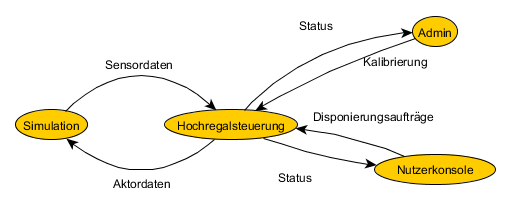
\includegraphics[width=\textwidth]{DFD/kontextdiagramm.png}
	\caption{Kontextdiagramm}
	\label{fig1}
\end{figure}
Aus dem Kontextdiagramm lässt sich leicht erkennen, dass das System aus zwei großen Teilen besteht. Auf der einen Seite ist die HRL-Steuerung, welche Eingaben erfasst, kontrolliert und die gewünschte Reaktion darauf berechnet. Auf der anderen Seite steht die Simulation, die für die physikalischen Abläufe nötige Zeit und das auslösen der diversen Sensoren simuliert. Verbunden sind beide durch diverse MessageQueues und eine globale Variable, welche in den weiteren Datenflussdiagrammen erleutert werden.
\subsubsection{DFD1 Simulation}
\begin{figure}[H]
	\centering
  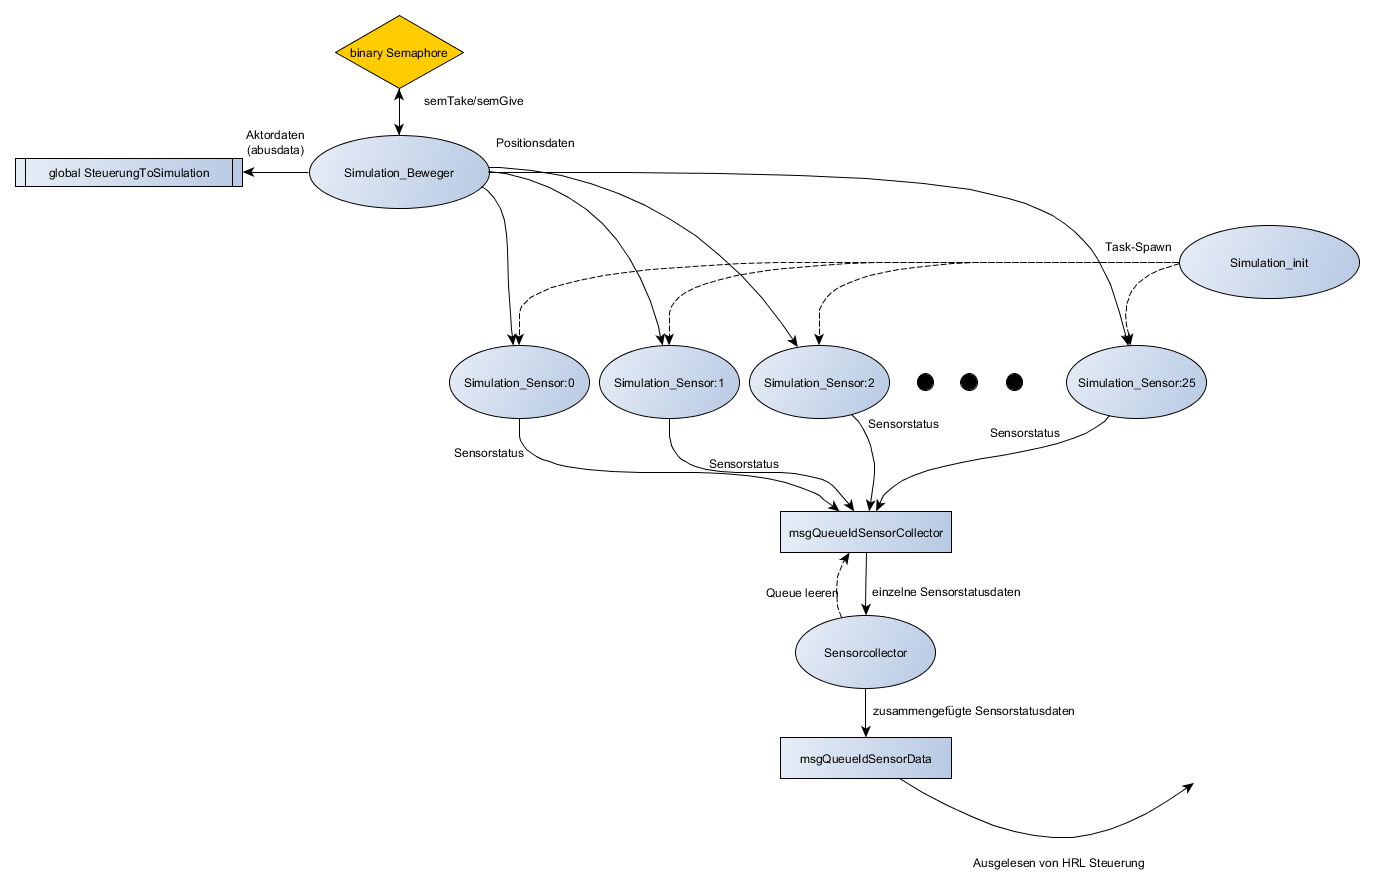
\includegraphics[width=\textwidth]{DFD/dfd1_simulation1_1.png}
	\caption{DFD1 Simulation}
	\label{fig2}
\end{figure}


\begin{figure}[H]
	\centering
  \includegraphics[width=\textwidth]{diagrams/gand.png}
	\caption{Gantt Diagramm der Task der Simulation}
	\label{gantt}
\end{figure}

Alle Tasks in der Simulation haben eine Priorität von 200 und ändern diese nicht. Sie werden in einer festen Reihenfolge erzeugt und laufen dann in jedem Zyklus in dieser Sequenz.\\
\\

\underline{Mini-Spec Simulation Beweger:}\\
Wie in Abb.\ref{gantt} zu sehen ist läuft der Beweger als erster Task eines Simulationsschrittes.
Der Beweger setzt virtuelle Position(Positionsdaten) nach Aktordaten (abusdata), welche durch einen Semaphore geschützt werden.  Da die Simulation minimal blockiert werden soll implementiert die Semaphore eine Prioritätsvererbung.\\ \\


\underline{Mini-Spec Simulation Sensor:}\\
Jeder Sensor bekommt eine ID die der Bitstelle in Sensorbits entspricht. Zur Initialisierung errechnet er so seine Position (\textit{triggeroffset}).\\ \\

\underline{Mini-Spec Simulation Sensor 0-22:}\\
Der Sensor Task berechnet das eigene \textit{triggeroffset} und gleicht dieses mit der virtuellen Position ab.\\
if(virtuelle Position-X == triggeroffset-X) true und eigene ID in \textit{msgQueueIdSensorCollector\\}
else false und eigene ID in \textit{msgQueueIdSensorCollector\\} \\
analog für Y- und Z-Sensoren\\ \\

\underline{Mini-Spec Simulation Sensor 23-24:}\\
Bei Sensoren für Lichtschranken wird die Berechnung nicht über ein \textit{triggeroffset}, sondern über Zeitkonstanten, welche hoch bzw. runter gezählt werden gesteuert.\\

\underline{Mini-Spec Simulation Sensor 25:}\\
Der Lichttaster wird gesetzt wenn er eine Auflade- bzw. Abladeoperation detektiert. Diese besteht (wie in Abb. \ref{fig3} zu sehen) aus unter den Ablagepunkt fahren, den Arm nach außen bzw. innen fahren und dann anheben, bzw. über den Ausgabepunkt fahren, den Arm nach außen bzw innen fahren und danach absenken.\\ \\
Setzen bzw. Entfernen eines Klötzchens aus bzw. in einen Lichttaster:\\ \\
if(Z = in Regal und Y= hoch) \\
Auslagerungsvorgang in Regal erkannt -> Lichttaster anschließend bedeckt und Belegungsmatrix[X][Y]= nicht belegt\\
\\
if(Z = in Regal und Y= runter)\\
Einlagerungsvorgang in Regal erkannt -> Lichttaster anschließend nicht bedeckt und Belegungsmatrix[X][Y] = belegt \\
\\
\\
if(Z = aus Regal heraus und Y= hoch)\\
Aufnahmevorgang in Eingabe-Slot erkannt -> Lichttaster anschließend bedeckt und Zeitkonstante von Lichtschranke in Slot wird zurückgesetzt\\
\\
if(Z = aus Regal heraus und Y= runter)\\
Auslagerungsvorgang in Ausgabe-Slot erkannt -> Lichttaster anschließend nicht bedeckt  Zeitkonstante von Lichtschranke in Slot wird zurückgesetzt\ \\
\\
\\
\underline{Mini-Spec Sensorcollector:}\\
Der Sensorcollector läuft nach allen Sensoren. Er  greift die Messwerte der einzelnen Sensoren aus \textit{msgQueueIdSensorCollector} ab (leeren der Queue) und fügt sie zu \textit{sbusdata} zusammen und schiebt diese in \textit{msgQueueIdSensorData}.\\ 


\subsubsection{DFD1 Steuerung}
\begin{figure}[H]
	\centering
  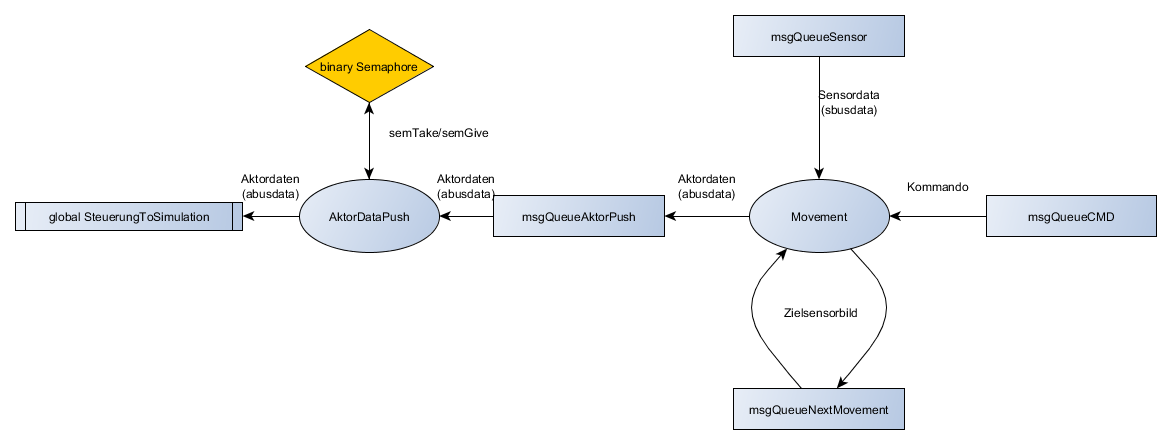
\includegraphics[width=\textwidth]{DFD/dfd1_steuerung.png}
	\caption{DFD1 Steuerung}
	\label{fig3}
\end{figure}

\underline{Mini-Spec Movement:}\\
Der Movement-Task fragt kontinuierlich nach einem neuem Auftrag aus der \textit{msgQueueCMD}, ist keiner da wird ein Timeout ausgelöst und das System geht in den Pause-Modus bzw. Zusatzaufgabe über. Wenn der Auftrag bereitsteht wird die Belegung geändert(für Befehle vsetspace und clearspace) bzw. es werden die acht Teilsensorbilder generiert(Befehle insert und remove). Diese werden in die \textit{msgQueueNextMovement} weitergeleitet und anschließend nacheinander aus der Queue abgearbeitet. Für jeden Teilauftrag wird auf neue Sensordaten aus \textit{msgQueueSensor} gewartet und die daraus entstehenden aktuellen Sensordaten mit den Soll-Sensordaten verglichen, dabei werden alle neuen Sensordaten auf ihre Legitimität überprüft und im Fehlerfall (z.B. blockierte Schiene) werden alle Motoren gestoppt und das System angehalten. Die Aktordoten werden in die \textit{msgQueueAktorPush} geleitet. \\

\underline{Mini-Spec AktorDataPush:}
\textit{AktorDataPush} dient zur Weitervermittlung der Aktordaten, welche geschützt weitergeleitet werden müssen(globale Variable),
wartet auf Aktordaten in der \textit{msgQueueAktorPush}. Sind Daten vorhanden wartet dieser auf die Semaphore, um anschließend in die globale Variable zu schreiben, aus welcher die Simulation liest. Für diese Semaphore wurde eine Prioritätsvererbung implementiert, um den Schreibvorgang auf die globale Variable möglichst nicht aus zu bremsen. \\
